\documentclass[a4paper]{article}

\usepackage{pgfplots}

\pgfplotsset{compat=1.3}

\begin{document}

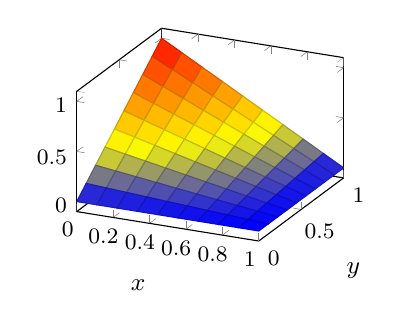
\begin{tikzpicture}
    \begin{axis}[footnotesize,xlabel=$x$,ylabel=$y$,unit vector ratio=]
    \addplot3[surf,samples=10,domain=0:1] {(1-x)*y};
    \end{axis}
\end{tikzpicture}
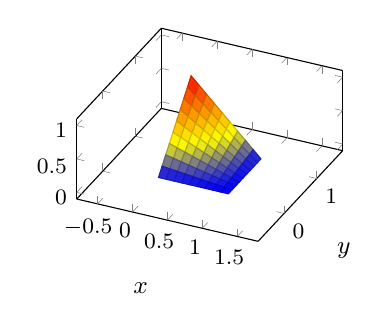
\begin{tikzpicture}
    \begin{axis}[footnotesize,xlabel=$x$,ylabel=$y$,unit vector ratio=1 1 1]
    \addplot3[surf,samples=10,domain=0:1] {(1-x)*y};
    \end{axis}
\end{tikzpicture}
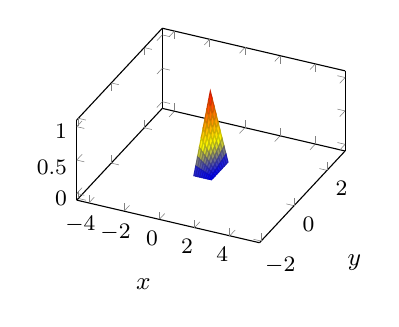
\begin{tikzpicture}
    \begin{axis}[footnotesize,xlabel=$x$,ylabel=$y$,unit vector ratio=0.25 0.5]
    \addplot3[surf,samples=10,domain=0:1] {(1-x)*y};
    \end{axis}
\end{tikzpicture}

\end{document}

